\documentclass[a4paper,14pt]{extarticle}
\usepackage{../../tex-shared/preamble}

\renewcommand{\mylabnumber}{2}
\renewcommand{\mylabtitle}{Расчет числовых характеристик и 
                           энтропии дискретной случайной величины}
\renewcommand{\mysubject}{Теория информационных процессов и систем}
\renewcommand{\mylecturer}{Заикина Е.Н.}

\begin{document}
\begin{titlepage}
    
    \thispagestyle{empty}
    
    \begin{center}
        
        Министерство науки и Высшего образования Российской Федерации \\
        Севастопольский государственный университет \\
        Кафедра ИС
        
        \vfill

        Отчет \\
        по лабораторной работе №\mylabnumber \\
        \enquote{\mylabtitle} \\
        по дисциплине \\
        \enquote{\MakeTextUppercase{\mysubject}}

    \end{center}

    \vspace{1cm}

    \noindent\hspace{7.5cm} Выполнил студент группы ИС/б-17-2-о \\
    \null\hspace{7.5cm} Горбенко К. Н. \\
    \null\hspace{7.5cm} Проверил \\
    \null\hspace{7.5cm} \mylecturer

    \vfill

    \begin{center}
        Севастополь \\
        \the\year{}
    \end{center}

\end{titlepage}
\section{Цель работы}
\begin{itemize}
    \item Изучение способов описания дискретных случайных величин.
    \item Приобретение практических навыков расчета числовых характеристик
          и энтропии дискретной случайной величины по ее закону распределения.
\end{itemize}

\section{Ход работы}
\begin{enumerate}
    \item Получить у преподавателя вариант задания.
    \item Написать функцию, определяющую распределение вероятностей
          дискретной случайной величины в соответствии с заданным
          законом распределения.
    \item Проверить условие нормировки.
    \item Написать функцию для определения начального момента s-го порядка.
          Выписать соответствующую формулу.
    \item Найти начальный момент нулевого порядка. Объяснить результат.
    \item Написать функцию для определения математического ожидания.
          Выписать соответствующую формулу.
    \item Построить графики зависимости математического ожидания от параметров
          распределения.
    \item Написать функцию для определения центрального момента s-го порядка.
          Выписать соответствующую формулу
    \item Найти центральный момент нулевого порядка. Объяснить результат.
    \item Найти центральный момент первого порядка. Объяснить результат.
    \item Написать функцию для определения дисперсии. Выписать
          соответствующую формулу.
    \item Построить графики зависимости дисперсии от параметров распределения.
    \item Написать функцию для определения среднеквадратического отклонения.
          Выписать соответствующую формулу.
    \item Построить графики зависимости среднеквадратического отклонения
          от параметров распределения.
    \item Написать функцию для определения коэффициента асимметрии. Выписать
          соответствующую формулу.
    \item Построить графики зависимости коэффициента асимметрии от
          параметров распределения.
    \item Написать функцию для определения коэффициента эксцесса.
          Выписать соответствующую формулу.
    \item Построить графики зависимости коэффициента эксцесса от параметров
          распределения.
    \item Построить графики распределения вероятностей для разных параметров
          распределения.
    \item Написать функцию, определяющую интегральный закон распределения 
          дискретной случайной величины, подчиненной заданному закону 
          распределения.
    \item Построить графики интегрального закона распределения для
          разных параметров распределения
    \item Написать функцию для вычисления энтропии.
    \item Построить графики зависимости энтропии от параметров распределения.
    \item Сделать развернутые выводы по результатам исследований.
\end{enumerate}

\section{Ход работы}
Задание ограничений, функции плотности вероятности, функции определения
начального момента порядка \code{s}, функции определения математического
ожидания, график зависимости математического ожидания от количества испытаний:
\begin{figure}[H]
    \centering
    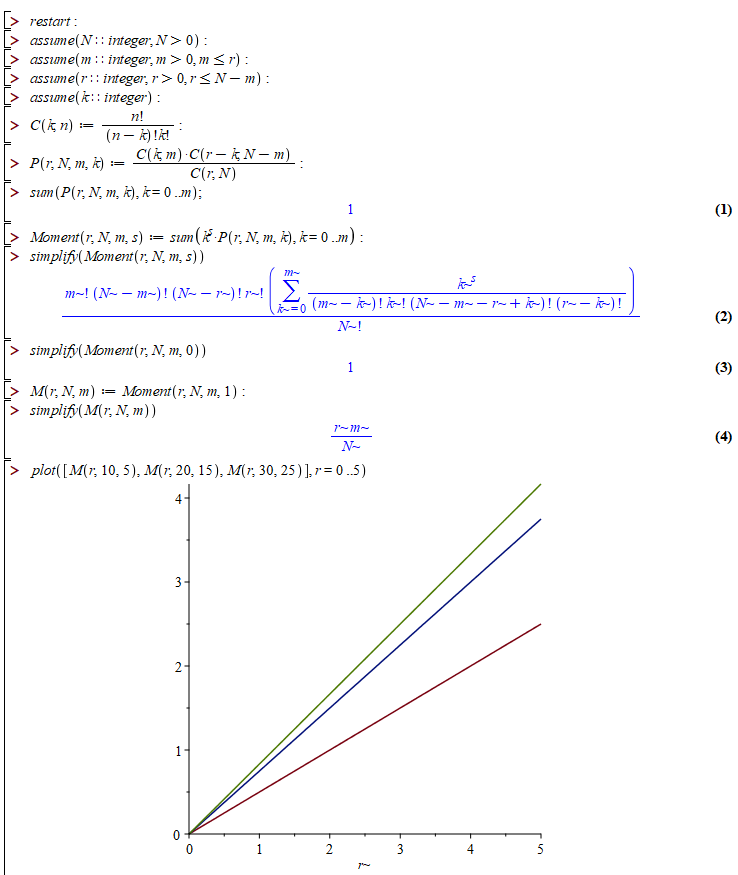
\includegraphics[width=\linewidth]{MO}
    \caption{График зависимости математического ожидания от количества испытаний}
\end{figure}
Функция определения центрального момента порядка \code{s}, дисперсии,
график зависимости дисперсии от количества испытаний:
\begin{figure}[H]
    \centering
    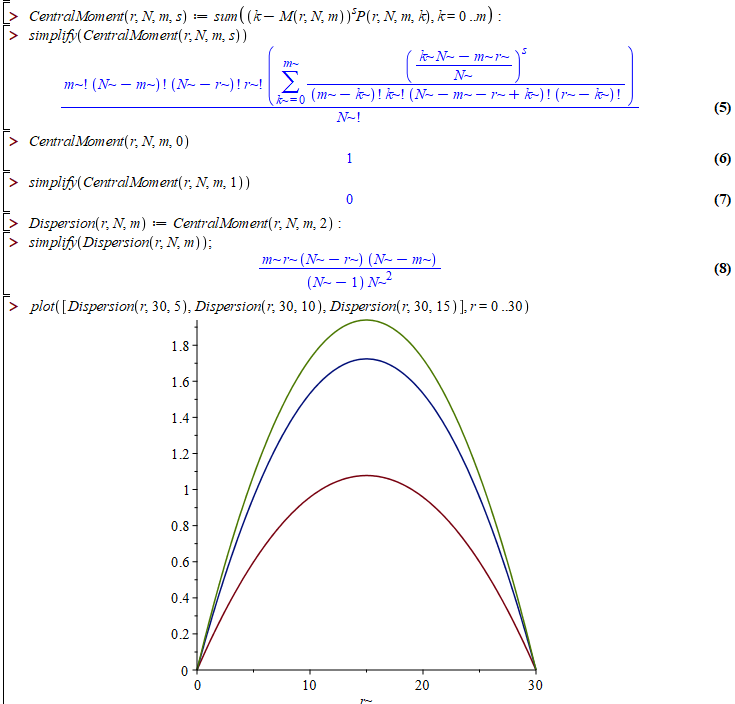
\includegraphics[width=\linewidth]{Dispersion}
    \caption{График зависимости дисперсии от количества испытаний}
\end{figure}
Функция определения среднеквадратического отклонения, график его заввисимости
от количества испытаний:
\begin{figure}[H]
    \centering
    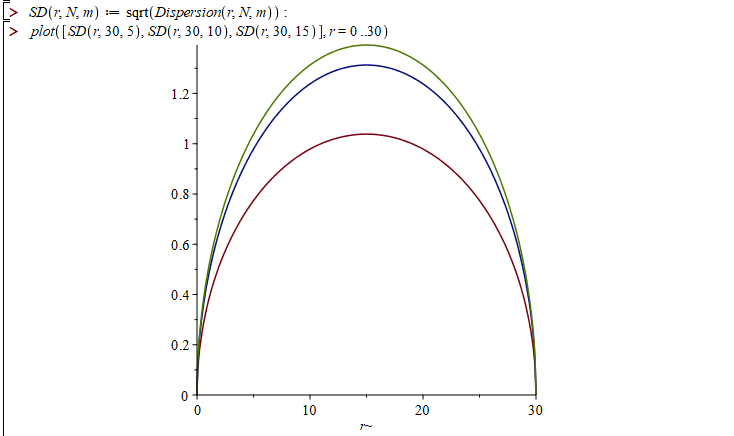
\includegraphics[width=\linewidth]{SD}
    \caption{График зависимости среднеквадратического отклонения
    от количества испытаний}
\end{figure}
Функция определения коэффициента ассиметрии, график его зависимости
от количества испытаний:
\begin{figure}[H]
    \centering
    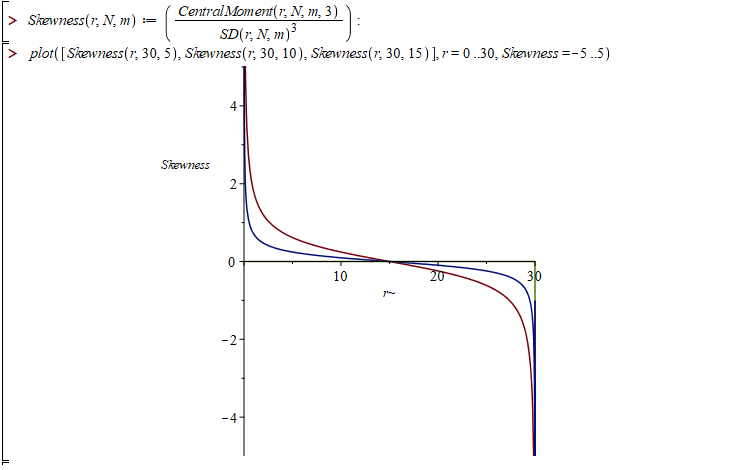
\includegraphics[width=\linewidth]{Skewness}
    \caption{График зависимости коэффициента ассиметрии
    от количества испытаний}
\end{figure}
Функция определения коэффициента эксцесса, график его зависимости
от количества испытаний:
\begin{figure}[H]
    \centering
    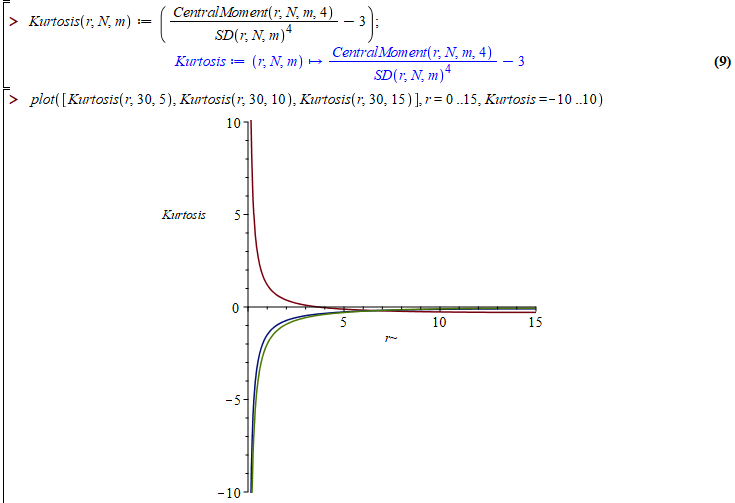
\includegraphics[width=\linewidth]{Kurtosis}
    \caption{График зависимости коэффициента эксцесса
    от количества испытаний}
\end{figure}
Графики зависимости функции распределения вероятностей от
количества испытаний:
\begin{figure}[H]
    \centering
    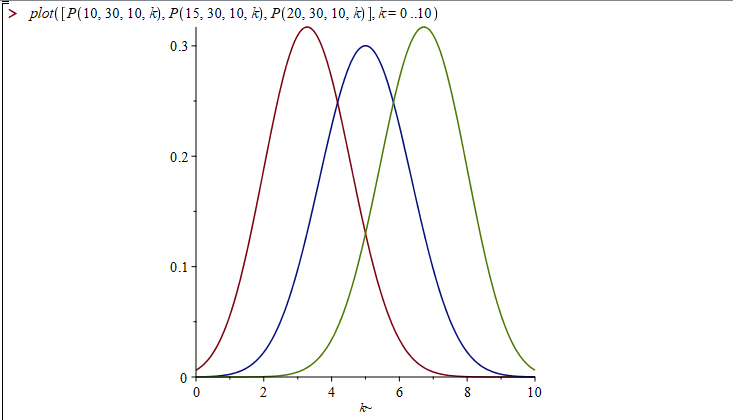
\includegraphics[width=\linewidth]{PDF}
    \caption{График зависимости функции плотности распределения
    от количества испытаний}
\end{figure}
График интегральной функции распределения:
\begin{figure}[H]
    \centering
    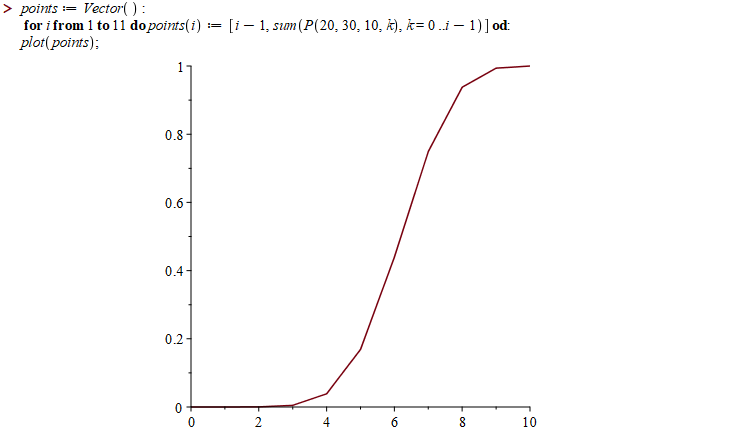
\includegraphics[width=\linewidth]{Integral}
    \caption{График интегральной функции распределения}
\end{figure}
Графики зависимости энтропии от количества испытаний:
\begin{figure}[H]
    \centering
    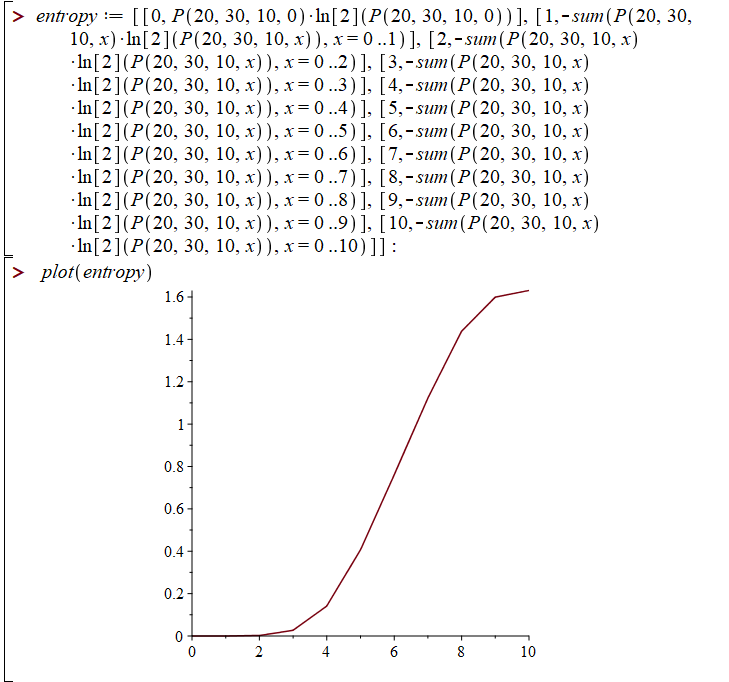
\includegraphics[width=\linewidth]{Entropy}
    \caption{График зависимости энтропии
    от количества испытаний}
\end{figure}
\section*{Выводы}
В ходе лабораторной работы было исследовано гипергеометрическое
распределение и его числовые характеристики. Параметрами
распределения являются: r - количество испытаний, N - количество
предметов в выборке, m - количесво предметов с искомым признаком
в выборке. Математическое ожидание зависит от всех параметров.
\end{document}